\chapter{System Design}
\label{cha:design}

This chapter presents the design of the end-to-end system. We first introduce the Cached Context concept that organizes prompts so that the backend cache engine can exploit reuse opportunities (Section~\ref{sec:design_cc}). We then describe the system architecture, with emphasis on the backend serving path that constitutes our central contribution and a brief account of the frontend that feeds it (Section~\ref{sec:design_arch}). Section~\ref{sec:design_backend_enh} details the backend enhancements that adapt CacheBlend's reference implementation to agentic workloads. Section~\ref{sec:design_frontend_impl} covers the implementation details on the frontend side that are needed to complete the end-to-end pipeline.

\section{Cached Context}
\label{sec:design_cc}

Cached Context is a prompt-organization concept \rashmi{This is basically how to chunk the gathered context, is it not? Is this a new concept or an existing one? Add references to this. If it is new, we need to chat about how to update the writing about this, we should consider bringing it up more clearly in intro for example. But then we will also have to have an evaluation to show the benefits and how exactly we do, that is at least a discussion on different approaches to do it. We will need a longer discussion on this. Let us discuss in our next meeting.} rather than a caching mechanism on its own. The key idea is to chunk each prompt at a per-context-object granularity, where a context object corresponds to a code snippet containing a symbol definition, a repository structure tree, or another semantically coherent unit of context. The actual caching is performed by the backend, which combines CacheBlend's content-addressed segment lookup with the position correction enhancement introduced in Section~\ref{sec:non_contiguous}. The two together make a cached chunk reusable regardless of its position in subsequent prompts, which is what we refer to as \emph{position-independent caching}.
Cached Context is a prompt-organization concept \rashmi{This is basically how to chunk the gathered context, is it not? Is this a new concept or an existing one? Add references to this. If it is new, we need to chat about how to update the writing about this.  and being proposed here, it is good to bring it up more clearly in intro but then we will also have to have an evaluation to show the benefits and how exactly we do, that is at least a discussion on different approaches to do it.} rather than a caching mechanism on its own. The key idea is to chunk each prompt at a per-context-object granularity, where a context object corresponds to a code snippet containing a symbol definition, a repository structure tree, or another semantically coherent unit of context. The actual caching is performed by the backend, which combines CacheBlend's content-addressed segment lookup with the position correction enhancement introduced in Section~\ref{sec:non_contiguous}. The two together make a cached chunk reusable regardless of its position in subsequent prompts, which is what we refer to as \emph{position-independent caching}.

To illustrate why this\rashmi{ What does "this" refer to here?} matters, consider the following example. Suppose the agent constructs a prompt after context retrieval, consisting of four parts: system instructions, repository structure, issue description, and a block of relevant code snippets. A naive chunking strategy would treat this prompt as a single unit or divide it into four coarse blocks. With Cached Context, we further decompose the context blocks into finer-grained chunks. The relevant code snippets block, for example, might contain definitions for multiple symbols retrieved by RepoGraph, where each symbol definition is now its own cache chunk.

Now consider a subsequent prompt in the same workflow, but with slightly different localization and a partly different set of code snippets, while most symbols and other blocks remain the same. Under conventional prefix caching, the cache can be reused only when the overlapping content appears identically from the start of the prompt. With Cached Context paired with the backend's position-independent caching, each overlapping symbol definition is a cache hit regardless of where it appears in the new prompt. This is particularly valuable in agentic workflows, where the order and combination of context elements frequently varies across requests.

\section{System Architecture}
\label{sec:design_arch}

Figure~\ref{fig:system_arch} illustrates the overall architecture. The design prioritizes modularity, allowing each component to be developed and tested independently. The remainder of this section walks through the backend and frontend in that order.

\begin{figure}[H]
\centering
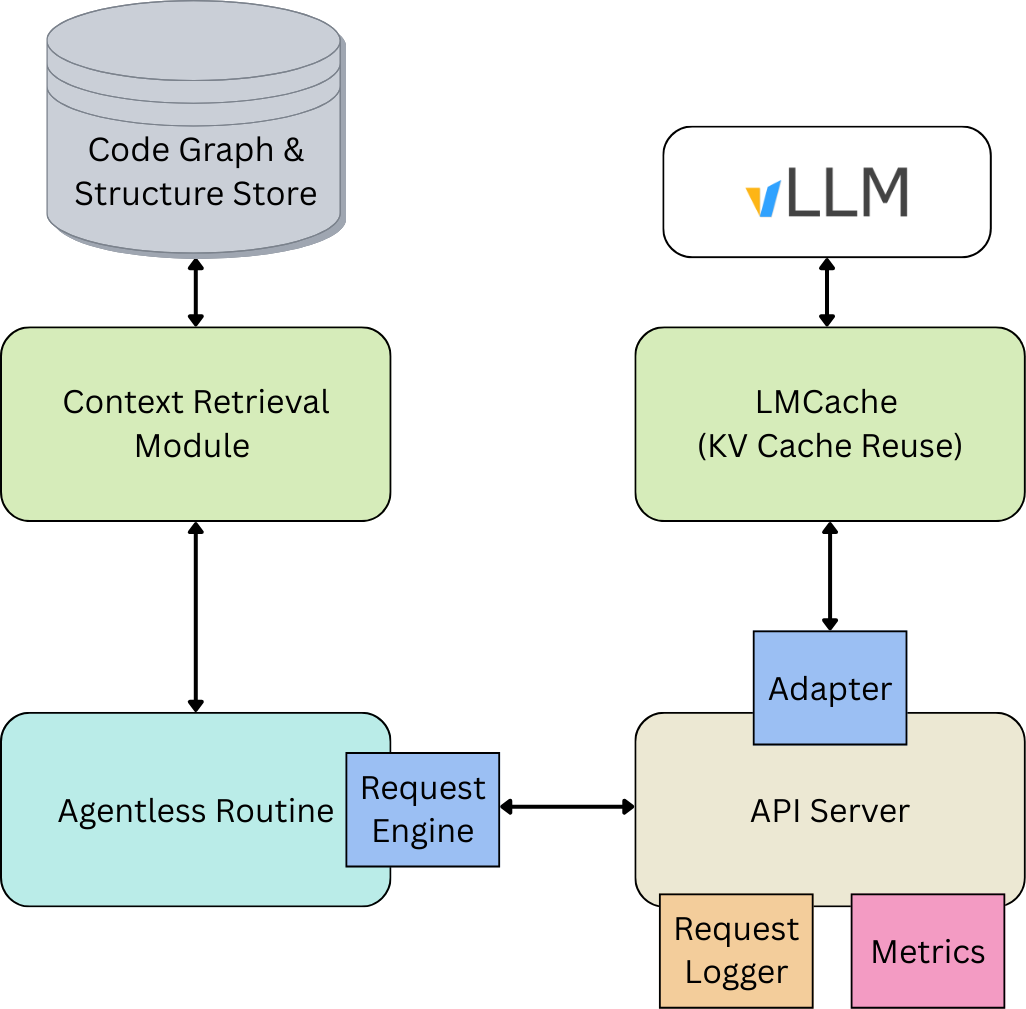
\includegraphics[width=0.75\linewidth]{graphs/E2E sys design.png}
\vspace{0.1in}
  \caption{\small End-to-end system architecture.}
 \label{fig:system_arch}
 \vspace{-0.15in}
\end{figure}

\subsection{Backend: API Server with CacheBlend}
\label{sec:design_arch_backend}

The backend consists of an API server that serves as the entry point for frontend requests. The server hosts the LLM inference engine (vLLM) with LMCache integration, which implements the CacheBlend algorithm for position-independent KV cache reuse. When a request arrives, the server performs the following steps:
\begin{enumerate}
    \item Parse the chat messages from the request.
    \item Pass the messages through the adapter module (described below) for tokenization and chunk extraction.
    \item Forward the processed prompt to the LLM engine with CacheBlend enabled.
    \item Return the generated response to the client.
\end{enumerate}

The backend exposes a chat-completion interface compatible with the OpenAI API format. This means any compatible frontend can drive the backend without modification beyond annotating context-object boundaries in its prompt templates.

\subsection{Adapter Module}
\label{sec:design_adapter}

The adapter module serves as the bridge between the frontend prompt format and the backend cache engine. Its responsibilities include:
\begin{enumerate}
    \item \textbf{Chunk extraction}: identifying and retrieving individual context objects from the incoming chat messages.
    \item \textbf{Tokenization}: encoding each chunk using the model's tokenizer, including correct handling of models with custom tokenization schemes (e.g., Devstral).
    \item \textbf{Chunk stitching}: reassembling the tokenized chunks to produce the final prompt token sequence consumed by the LLM engine.
\end{enumerate}

The adapter's design supports flexible chunking granularity based on the frontend prompt template and user preference. If chunking is per symbol, the frontend adds a delimiter after each code snippet fetched during code graph exploration. If a coarser granularity is desired (e.g., per context block), delimiters can be placed only between major sections of the prompt. This flexibility makes the system robust to various workload patterns and to differing optimal chunk sizes.

\subsection{Frontend: RepoGraph + Agentless}
\label{sec:design_arch_frontend}

We use RepoGraph as the frontend context retrieval algorithm, integrated with the Agentless procedural framework. Agentless follows a three-step routine:
\begin{enumerate}
    \item \textbf{Localize}: given an issue description, identify the files and code regions most likely to require modification.
    \item \textbf{Repair}: generate candidate patches for the localized regions.
    \item \textbf{Rerank}: evaluate and rank the candidate patches, selecting the most promising one for submission.
\end{enumerate}

RepoGraph enhances the localization phase by providing repository-aware context. Rather than relying solely on file-level search, Agentless can query RepoGraph's code graph to retrieve symbol definitions, call chains, and structural information. This integration ensures that the LLM receives semantically complete context. For example, when localizing a bug in a function, the model also receives definitions of the symbols referenced by that function.

To enable Cached Context, we modify Agentless's prompt generation routine to make context object boundaries explicit, which exposes chunk boundaries to the backend adapter without affecting the semantic content of the prompt. The frontend is otherwise treated as a pluggable component: any retrieval module that produces prompts with explicit chunk boundaries can replace RepoGraph + Agentless without changes to the backend.

\section{Backend Enhancements}
\label{sec:design_backend_enh}

This section presents the backend enhancements that adapt CacheBlend's reference implementation (LMCache) to the workload characteristics of code agents. Each targets one of the limitations identified in Section~\ref{sec:bg_kvcache}: position correction for chunks reused at a new offset, lock contention and deadlocks in memory allocation, and the lack of fine-grained diagnostic instrumentation. The last of these is presented together with the request logging and replay mechanism, since the two jointly provide the measurement basis for the latency evaluation in Chapter~\ref{cha:eval}.

\subsection{Position Correction for Non-Contiguous Reuse}
\label{sec:non_contiguous}

The segment token database used in CacheBlend's blend mode already hashes each chunk by its own content (independent of position). Cache lookup is therefore content-addressed: a chunk that appeared in a prior request can be matched again in any later request regardless of where it now sits in the prompt. For example, if prompt $A$ contains the ordered chunks $[C_1, C_3, C_4]$ and a later prompt $B$ contains $[C_2, C_3, C_4]$, the segment-level lookup correctly identifies $C_3$ and $C_4$ as cache hits in $B$ even though $C_2$ replaced $C_1$ at the start. This much works in upstream LMCache.

The runtime path that actually uses these hits, however, is incomplete in upstream. When a cached chunk is loaded back onto the GPU at a position different from where it was originally cached, the rotary positional embeddings stored in the KV must be corrected for the new position. The layerwise GPU connector implements this correction by reading \texttt{memory\_obj.metadata.old\_positions} at load time and calling a fused rotary kernel. The upstream \texttt{MemoryObjMetadata}, however, does not define the \texttt{old\_positions} field, so the path raises an attribute error as soon as position correction is exercised. The effect is that only chunks reused at their original positions are usable in practice, which is precisely the contiguous case.

We add the \texttt{old\_positions} field to \texttt{MemoryObjMetadata} along with its serialization and deserialization handlers, and we populate it from the chunk's positions at save time. With this in place, a cached chunk can be loaded at any later position and the rotary embeddings are corrected accordingly. Returning to the example above, the cache hits for $C_3$ and $C_4$ in prompt $B$ are now usable even though $C_3$ and $C_4$ may sit at different positions in $B$ than they did in $A$ (therefore $[C_1, C_3, C_4]$ -> $[C_2, C_4, C_3]$ also hits 2 out of 3 chunks). The change preserves backward compatibility: a chunk that happens to be reused at its original position incurs an identity correction. In multi-turn agentic workloads where context objects are reordered or partially substituted between requests, this completes the non-contiguous reuse path that CacheBlend's content-addressed lookup was already pointing toward.

\subsection{Enhanced Memory Allocation and Locking}
\label{sec:mem_alloc}

The cache engine's hot storage tier is an in-memory CPU buffer (the \texttt{LocalCPUBackend}), which holds KV chunks before they are loaded back onto the GPU. All allocation and eviction in the path discussed below operates on this in-memory tier; no disk-backed storage is involved. Scaling CacheBlend to agentic workloads with high request concurrency and large prompt lengths exposed two bottlenecks in this tier's memory management path.

\paragraph{Batched varied-shape allocation.}
Each cache chunk corresponds to a memory object whose shape depends on the chunk's token count. The original implementation allocated these objects one at a time, acquiring and releasing the CPU buffer lock for each chunk. Under high concurrency, this per-chunk locking becomes a serialization bottleneck: a single store operation for a prompt comprising $N$ chunks requires $N$ lock acquisitions. We introduce a \texttt{batched\_allocate\_varied} method that accepts a list of shapes in one call, acquires the lock once, performs all allocations (with bulk eviction if capacity is exceeded), and releases the lock. This reduces lock contention by a factor of $N$ per request and avoids partial-allocation states where some chunks succeed while others fail due to concurrent eviction.

\paragraph{Bounded eviction with deadlock prevention.}
When the in-memory cache is full, the allocator must evict existing entries to make room. In the original design, the eviction loop retried indefinitely until sufficient space was freed. Under heavy concurrent load, this could deadlock: if all cache entries were pinned by in-flight lookups on other threads, no entry was eligible for eviction, and the allocator would spin indefinitely while holding the CPU buffer lock. We bound the eviction loop to a configurable maximum number of retries (\texttt{MAX\_EVICTION\_RETRIES}). If the limit is reached, the allocation fails gracefully and the request falls back to full prefill computation, avoiding system-wide stalls.

\subsection{Debugging and Profiling Infrastructure}
\label{sec:profiling}
\label{sec:request_logging}

Diagnosing why a given request did or did not benefit from cache reuse requires visibility at two levels: what the cache engine spent its time on inside a request, and what sequence of requests the agent produced in the first place. We implement one subsystem for each, and together they form the measurement basis for the latency evaluation in Chapter~\ref{cha:eval}.

\paragraph{Per-request profiling.}
To enable fine-grained latency analysis of the cache engine under realistic workloads, we implement a per-request profiling module that instruments the critical path through the adapter, cache engine, storage backend, and GPU connector. The profiler is organized around two abstractions: \emph{operations}, which correspond to logical units of work (e.g., a single request's retrieve pass), and \emph{phases}, which subdivide an operation into timed intervals (e.g., token database lookup, per-layer storage retrieval, per-layer GPU onload).

The profiler uses thread-local storage to maintain a per-thread operation stack, ensuring that timing records from tensor-parallel workers do not bleed across threads. Each phase is recorded with its wall-clock duration, parent operation identifier, and thread ID. On completion, the profiler emits per-operation summaries in JSONL format, enabling post-hoc aggregation and visualization.

Figure~\ref{fig:profiler_timeline} shows an example timeline produced by the profiler during a CacheBlend-enabled serving session. Each point represents a single profiled operation, plotted by wall-clock time on the x-axis and measured latency on the y-axis, and color-coded by operation type. The \texttt{retrieve\_layer} operations (orange) dominate the per-step cost on the read path, typically clustering between 25 and 75\,ms with occasional spikes above 100\,ms. The \texttt{store\_layer} operations (green) cover the synchronous GPU-to-CPU offload of newly computed KV states, which Section~\ref{sec:rec_miss_penalty} identifies as the dominant cost whenever the cache misses. The \texttt{adapter.start\_load\_kv} markers (red, near the baseline) indicate the lightweight entry point into the cache path. This visualization enables rapid identification of latency outliers and temporal patterns that would be invisible in aggregate statistics.

\begin{figure}[H]
\centering
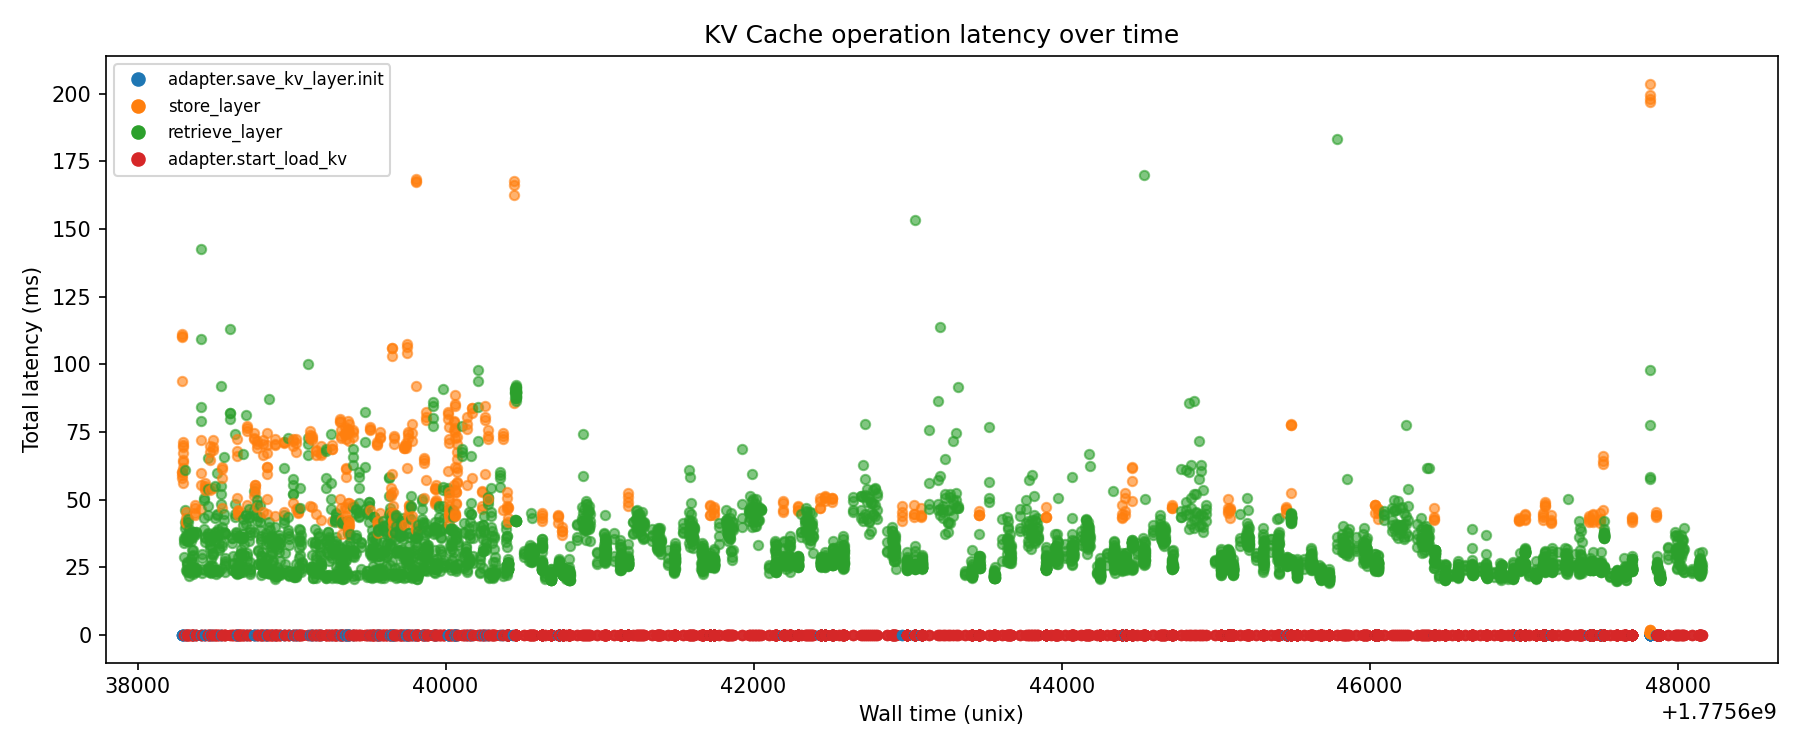
\includegraphics[width=\linewidth]{graphs/lmcache_profile_20260408_044806_advprof_chunklb128_timeline.png}
\vspace{-0.1in}
  \caption{\small Example profiler output: per-operation latency timeline during a CacheBlend-enabled serving session (chunk lower bound 128 tokens). Each point is a single profiled operation, color-coded by type. The clustering of \texttt{retrieve\_layer} (orange) at 25--75\,ms reflects the roughly token-independent per-call retrieve cost analyzed in Section~\ref{sec:variance_analysis}; the token-proportional store cost is analyzed in Section~\ref{sec:rec_miss_penalty}.}
 \label{fig:profiler_timeline}
 \vspace{-0.15in}
\end{figure}

This instrumentation is what makes performance anomalies visible at all. It revealed both the source of the speedup variance among small requests (Section~\ref{sec:variance_analysis}) and the synchronous KV store path that dominates the penalty on cache misses (Section~\ref{sec:rec_miss_penalty}). Neither would have been visible from end-to-end TTFT measurements alone.

\paragraph{Request logging and replay.}
To support debugging and reproducible experimentation, the API server includes a request logging module. During a server session, all incoming requests and their corresponding responses are captured and stored as a local trace file.

This transparency enables inspection of which stage during the Agentless routine may have caused a performance bottleneck. For example, if localization prompts consistently exhibit low cache hit rates, the prompt template can be adjusted to improve context alignment across requests.

In addition, the server supports a \textbf{replay} functionality that parses requests from any trace file and simulates the workload internally. This feature enables:
\begin{itemize}
    \item Evaluation on captured traces from real agentic workloads without re-running the full agent pipeline.
    \item Modularized testing through synthetic small traces that exercise specific caching scenarios.
    \item A/B comparison of different caching configurations on identical workloads.
\end{itemize}

These capabilities are essential for the latency evaluation methodology in Chapter~\ref{cha:eval}. The replay mechanism lets us drive the backend with a fixed, deterministic trace under both blend and no-blend configurations, eliminating the variability that would otherwise come from re-running the agent loop end-to-end.

\section{Frontend Integration Details}
\label{sec:design_frontend_impl}

Beyond the core architecture, several implementation details on the frontend side improve the system's robustness and the realism of the prompts that reach the backend.

\subsection{Context Truncation}
\label{sec:context_truncation}

For complex coding tasks involving multiple files and nested dependencies, the frontend can exceed the model's token limit when constructing a prompt. Originally, prompts were naively truncated at the end when the token limit was reached. This approach frequently results in important instructions (such as output format requirements or validation criteria) being omitted from the prompt. Even when the LLM receives sufficient context to understand the problem, it may underperform due to missing instructions.

Our solution leverages the model's tokenizer to calculate the token length of each context block and the prompt template. Before constructing the prompt, the last context block is truncated to exactly fit the remaining token budget, so that the critical pieces on the template stay intact and instructions are passed to the LLM as desired. This improves the reliability of the generated patches when the context is long.

\subsection{Local Store for Precomputed Data}
\label{sec:local_store}

Computing the code graph and repository structure from scratch for every task instance incurs significant latency overhead. RepoGraph's graph construction involves parsing all source files using \texttt{tree-sitter}, identifying symbol definitions and references, and building the dependency graph. For large repositories, this process can take several minutes.

To address this, we introduce a local store that caches these large data structures. The store is keyed by repository ID and commit hash, ensuring that cached data remain valid across tasks targeting the same codebase state. This optimization is particularly valuable when processing multiple issues against the same repository (common in benchmark evaluations like SWE-bench) or when the same repository is revisited across different agent sessions.
